\section{Risposta direzionale di un tubo di Pitot}
Il tubo di Pitot è una sonda cilindrica con sezione trasversale circolare che viene utilizzata allineata con la corrente. Tale sonda è munita di una presa di pressione totale frontale e di una o più prese di pressione statica (solitamente quattro prese a novanta gradi tra loro) poste sulla superficie cilindrica ad opportuna distanza dall'estremità anteriore.\\\\
La sonda presenta al suo interno due tubi coassiali. In quello più interno si risente la pressione totale mentre sul tubo esterno sono posizionate le prese di pressione statica. All'estremità opposta alla zona di misura della sonda sono presenti due uscite corrispondenti al segnale di pressione statica e a quello di pressione totale, da collegare con un trasduttore di pressione.
\begin{figure}[h]
    \centering
    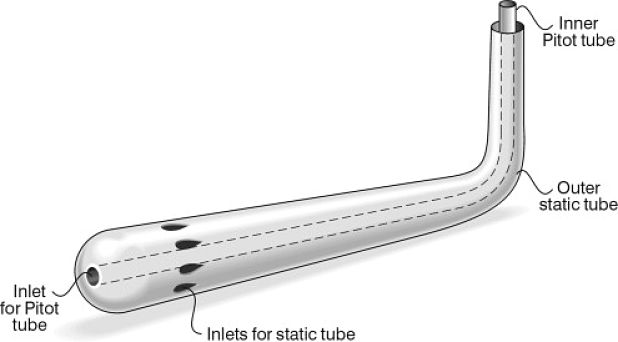
\includegraphics[width=0.55\linewidth]{images/2/pitotsketch.png}
    \caption{Rappresentazione di un tubo di Pitot}
\end{figure}

\subsection{Descrizione dell'esperimento}
La presente esercitazione si pone come obiettivo la caratterizzazione di una sonda di Pitot. In particolare si vuole:
\begin{itemize}
    \item Valutare l'effetto del disallineamento $\alpha$ della sonda sulla pressione totale, sulla pressione statica e sulla pressione dinamica;
    \item Determinare la velocità della corrente;
    \item Valutare l'effetto del numero di Reynolds.
\end{itemize}
\noindent La sonda di Pitot in esame possiede le seguenti caratteristiche geometriche:
\begin{itemize}
    \item Diametro esterno: $D = 3$ mm;
    \item Diametro interno: $d = 1$ mm;
    \item Distanza delle prese statiche dal bordo di attacco: $L_1 = 12.5$ mm;
    \item Distanza delle prese statiche dal gambo: $L_2 = 37$ mm.
\end{itemize}
\newpage
\noindent La valutazione della velocità della corrente si ricava considerando la relazione di Bernoulli:
\begin{equation*}
    p_0 = p + \frac12 \rho V^2 \quad \rightarrow \quad q = p_0 - p = \frac12 \rho V^2
\end{equation*}
Dalla velocità è possibile ricavare il numero di Reynolds della corrente:
\begin{equation*}
    Re = \frac{\rho V D}{\mu}
\end{equation*}
L'errore commesso nella misura delle pressioni in presenza di disallineamento viene valutato definendo prima una grandezza $\varepsilon$ che caratterizza l'entità dell'errore. Si possono pertanto introdurre tre funzioni ognuna riferita alle tre pressioni:
\begin{equation*}
    \varepsilon_{p_0}(\alpha) = \frac{p_0(\alpha) - p_{0,\alpha=0}}{q_{\alpha=0}} \qquad \varepsilon_{p}(\alpha) = \frac{p(\alpha) - p_{\alpha=0}}{q_{\alpha=0}} \qquad \varepsilon_{q}(\alpha) = \frac{q(\alpha) - q_{\alpha=0}}{q_{\alpha=0}}
\end{equation*}

\subsection{Catena di misura}
Analogamente alla precedente esercitazione, il flusso di riferimento per la caratterizzazione della sonda di Pitot è il cuore potenziale di un getto.\\\\
Il tubo di Pitot è connesso al trasduttore di pressione SETRA mod 239 C già precedentemente tarato ($K_t=550$ Pa/V). Per il calcolo della pressione dinamica ai due ingressi del trasduttore sono connessi i canali pneumatici relativi alla pressione totale ed alla pressione statica del tubo di Pitot. Per il calcolo della pressione totale, invece, il canale pneumatico relativo alla pressione statica del tubo di Pitot viene scollegato, così che il trasduttore riceva in ingresso la pressione ambiente. Per il calcolo della sola pressione statica, analogamente, viene scollegato il canale pneumatico relativo alla pressione totale del tubo di Pitot. In questo modo è possibile valutare la pressione totale, la pressione statica e la pressione dinamica nel cuore potenziale del getto.\\\\
Per operare il disallineamento controllato del tubo di Pitot, questo è montato su un goniometro, in modo tale che anche modificando l'angolo $\alpha$ di disallineamento la testa della sonda rimanga nella stessa posizione, il più possibile vicina all'asse del getto.\\\\
La catena di misura è dunque costituita da:
\begin{itemize}
    \item Getto;
    \item Tubo di Pitot, posizionato nel cuore potenziale del getto;
    \item Goniometro opportunamente posizionato;
    \item Trasduttore di pressione SETRA 239 C;
    \item Sistema di acquisizione dati (SAD) e PC con LabView.
\end{itemize}

\newpage
\begin{figure}[ht]
    \centering
    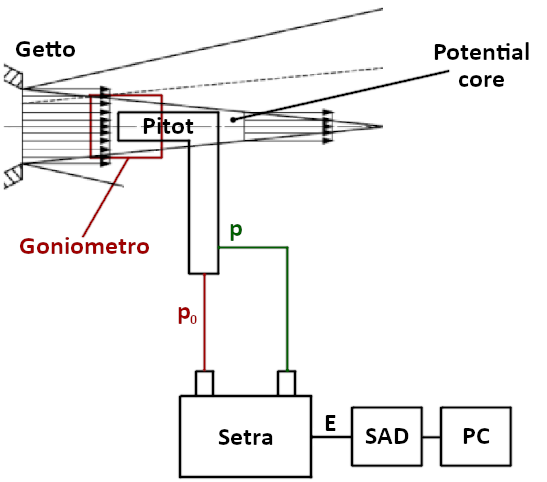
\includegraphics[width=.65\textwidth]{images/2/catena.png}
    \caption{Rappresentazione semplificata della catena di misura, con canali pneumatici in configurazione per la misura della pressione dinamica}
\end{figure}
\begin{figure}[h!]
    \centering
    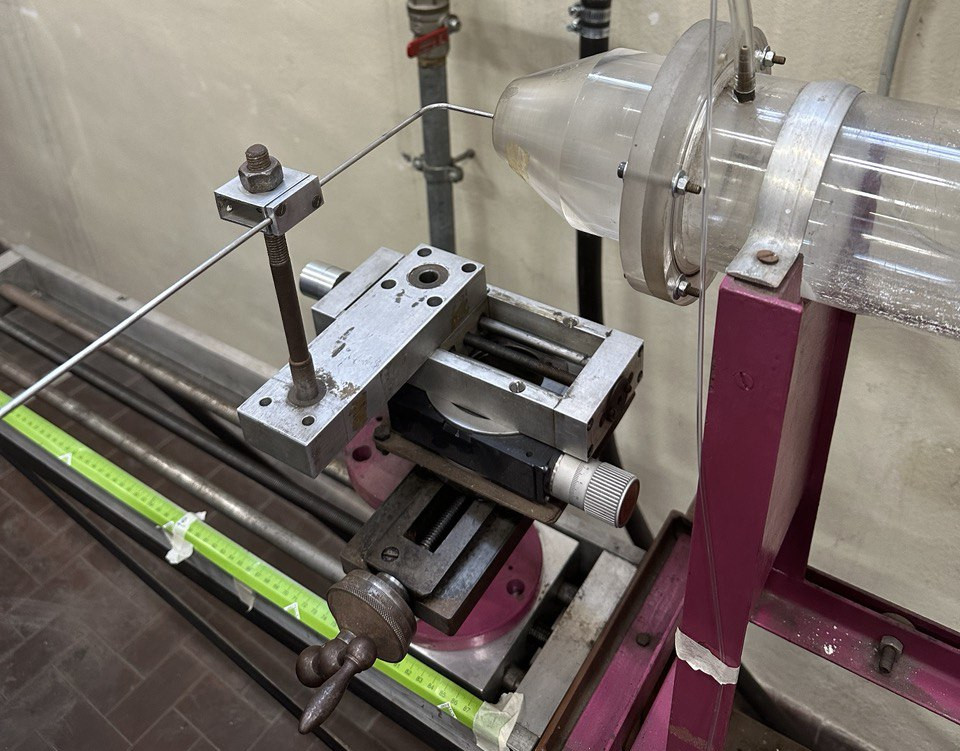
\includegraphics[width=.65\textwidth]{images/2/goniometro.jpg}
    \caption{Goniometro opportunamente posizionato}
\end{figure}

\newpage
\subsection{Procedura sperimentale}
Come prima operazione è necessario misurare la tensione di offset $E_0$, cioè la tensione in uscita al trasduttore quando non è applicata alcuna differenza di pressione. Per fare ciò, si acquisiscono i dati in uscita al trasduttore con il getto spento.\\\\
Una volta misurata tale tensione, si può scomporre il segnale in uscita come:
\begin{equation*}
    E(\Delta p) = E_0 + \Delta E(\Delta p)
\end{equation*}
Si procede mantenendo una portata costante per ogni squadra e quindi una velocità costante nel cuore potenziale del getto e variando l'angolo di disallineamento $\alpha$ in entrambi i versi di rotazione. Per ogni angolo $\alpha$, misurato tramite una scala graduata, si acquisisce il segnale elettrico di uscita corrispondente.\\\\
I dati sono acquisiti con una frequenza $f_s=2$ kHz per un periodo di $T=1$ s.\\\\
I dati grezzi acquisiti durante la procedura sono riportati in appendice \ref{a2}.

\subsection{Analisi dati}
L'analisi dati è condotta con l'ausilio di un codice Python, riportato in appendice \ref{b2}.\\\\
Per il calcolo della densità si utilizzano le condizioni di pressione e temperatura ambiente rilevate al momento delle misure, quindi:
\begin{equation*}
    \rho = \frac{p_{amb}}{R\,T_{amb}}
\end{equation*}
dove $R\approx 287$ J/kgK è la costante dei gas relativa all'aria.\\\\
Per il calcolo della viscosità dinamica $\mu$ si utilizza la legge di Sutherland:
\begin{equation*}
    \mu = 1.46\cdot10^{-6} \frac{T_{amb}^{3/2}}{T_{amb}+110}
\end{equation*}
Dai dati acquisiti si ricava la pressione dinamica "vera", cioè a disallineamento nullo $q_{\alpha=0}$ per ognuna delle quattro portate analizzate. Da tale grandezza si ricava la velocità:
\begin{equation*}
    V = \sqrt{\frac{2q_{\alpha=0}}{\rho}}
\end{equation*}
E quindi il numero di Reynolds:
\begin{equation*}
    Re = \frac{\rho V D}{\mu}
\end{equation*}
Infine si calcolano gli errori $\varepsilon$ per la pressione statica, la pressione totale e la pressione dinamica, utilizzando le formule precedentemente esplicitate.
\newpage
\noindent Si ottengono i seguenti diagrammi:
\begin{figure}[h!]
    \centering
    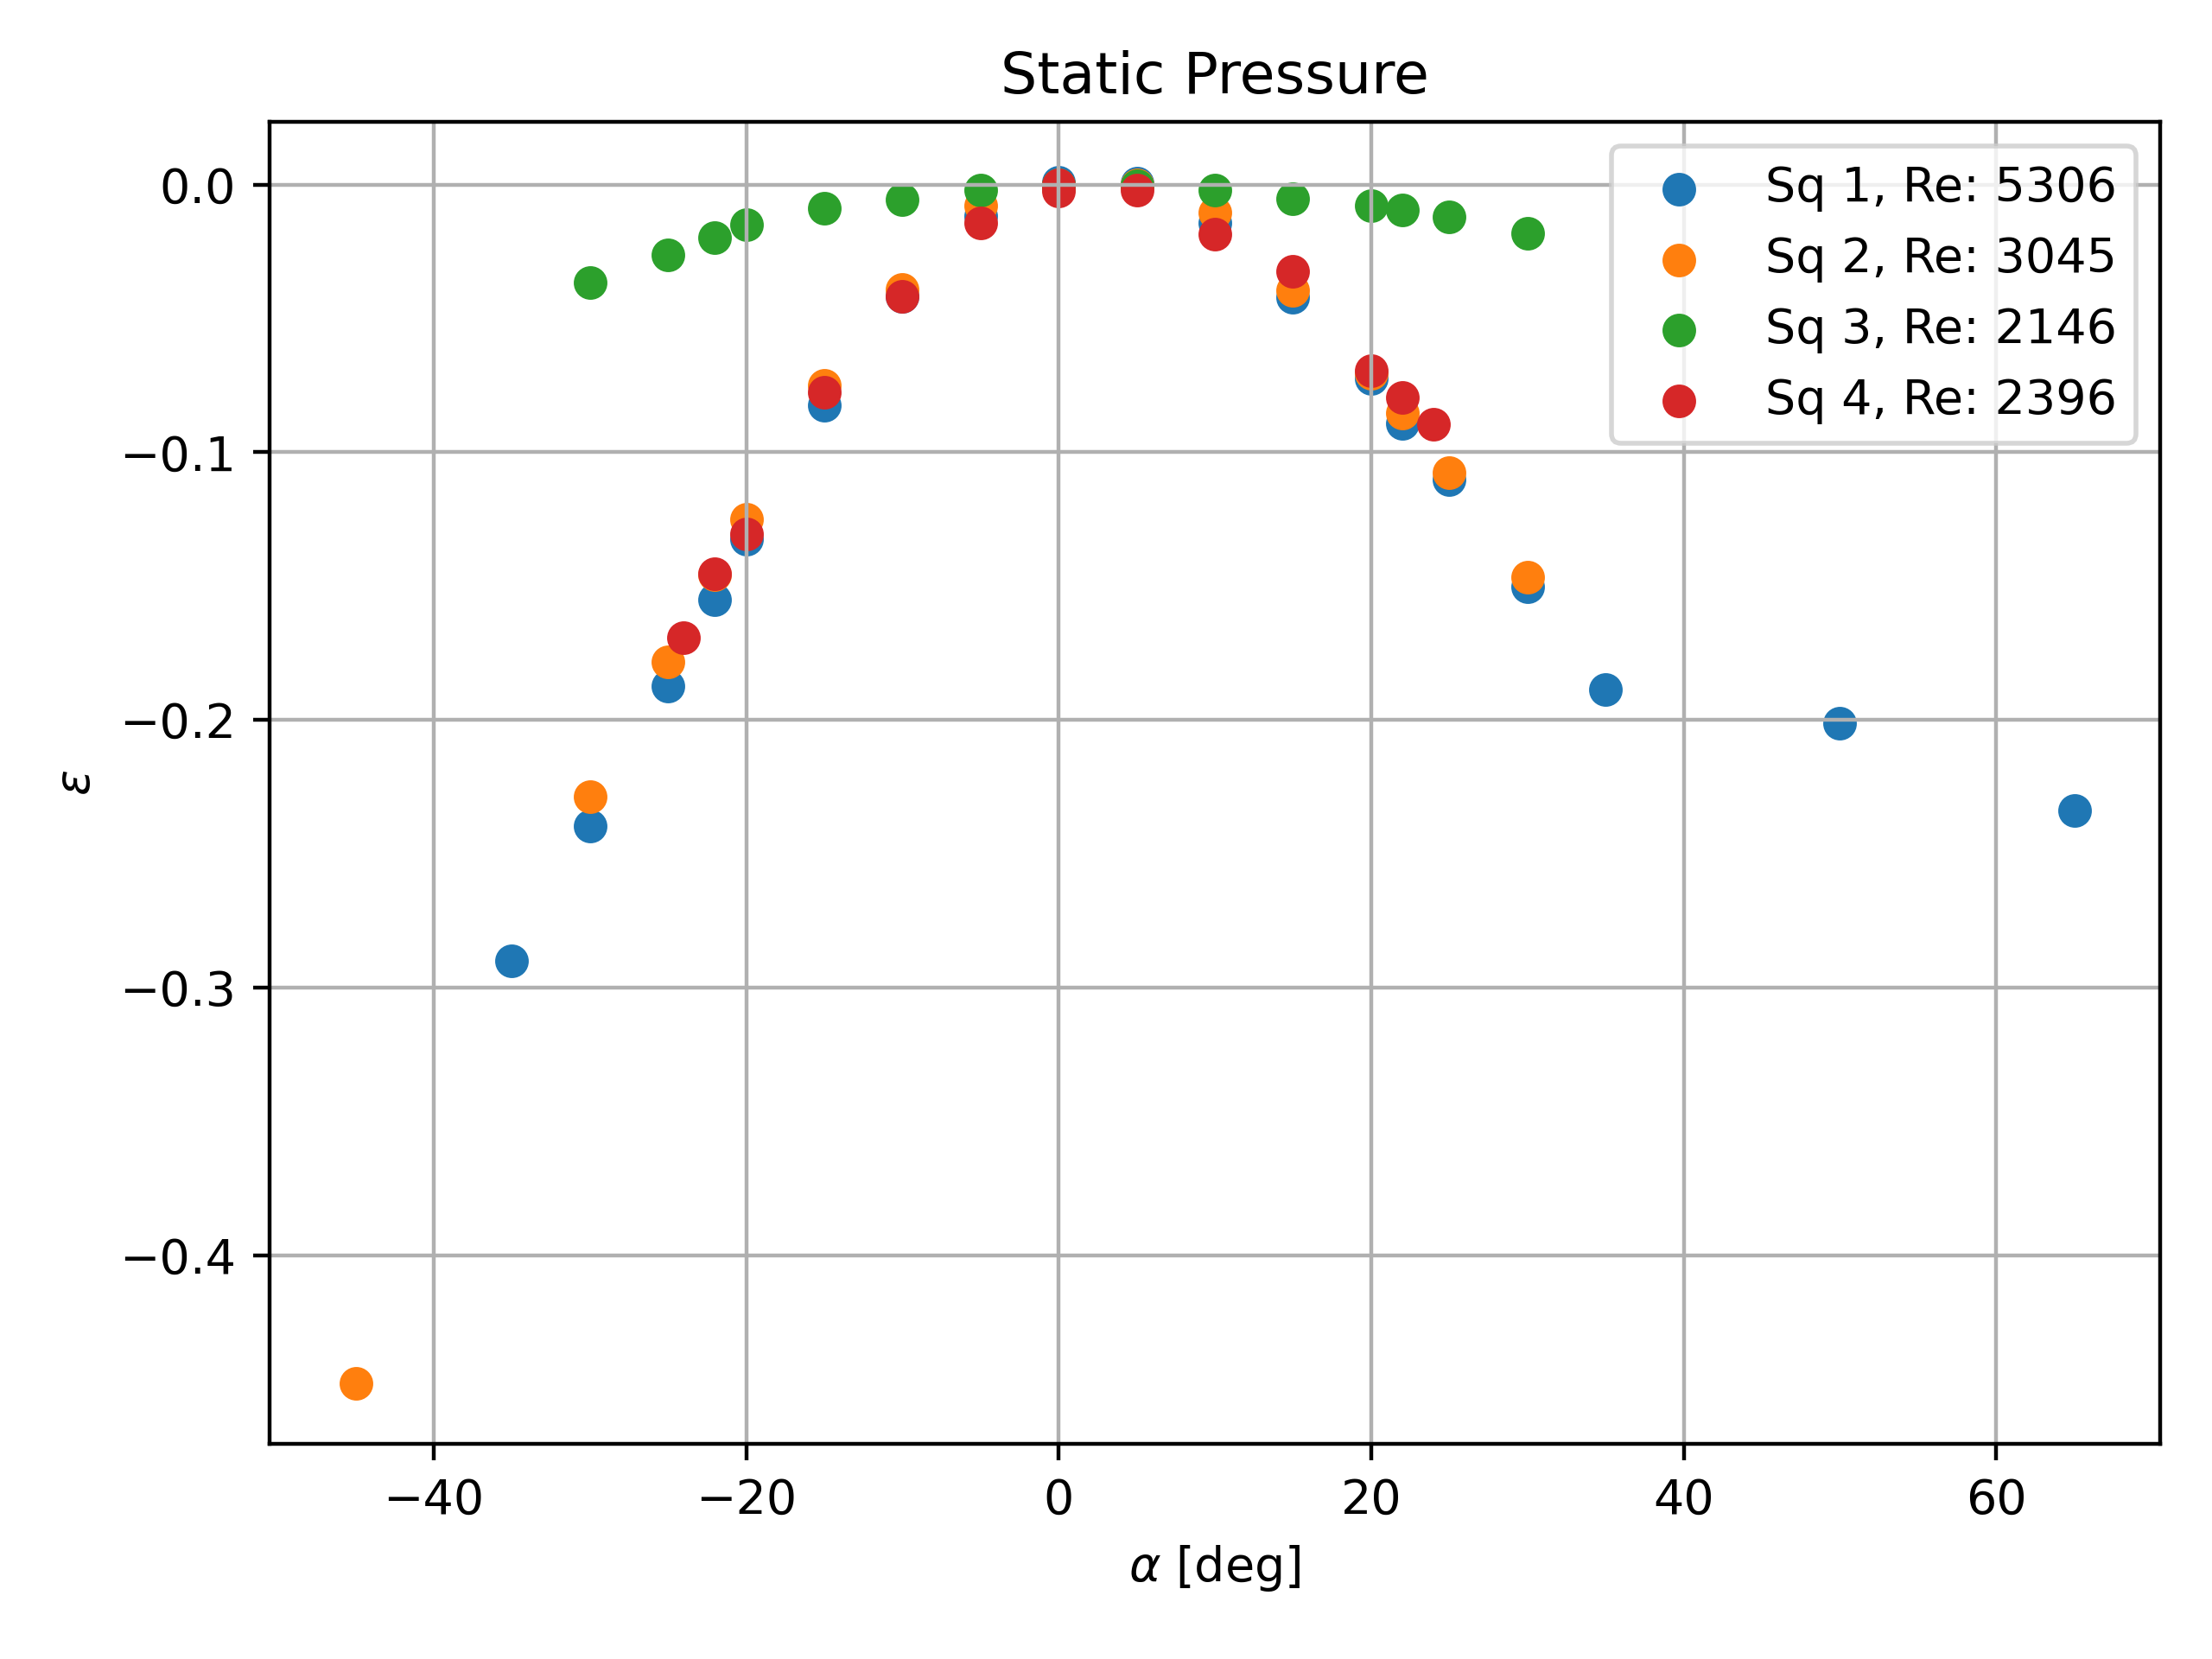
\includegraphics[width=.76\textwidth]{images/2/p.png}
    \caption{Pressione statica}
\end{figure}
\begin{figure}[h!]
    \centering
    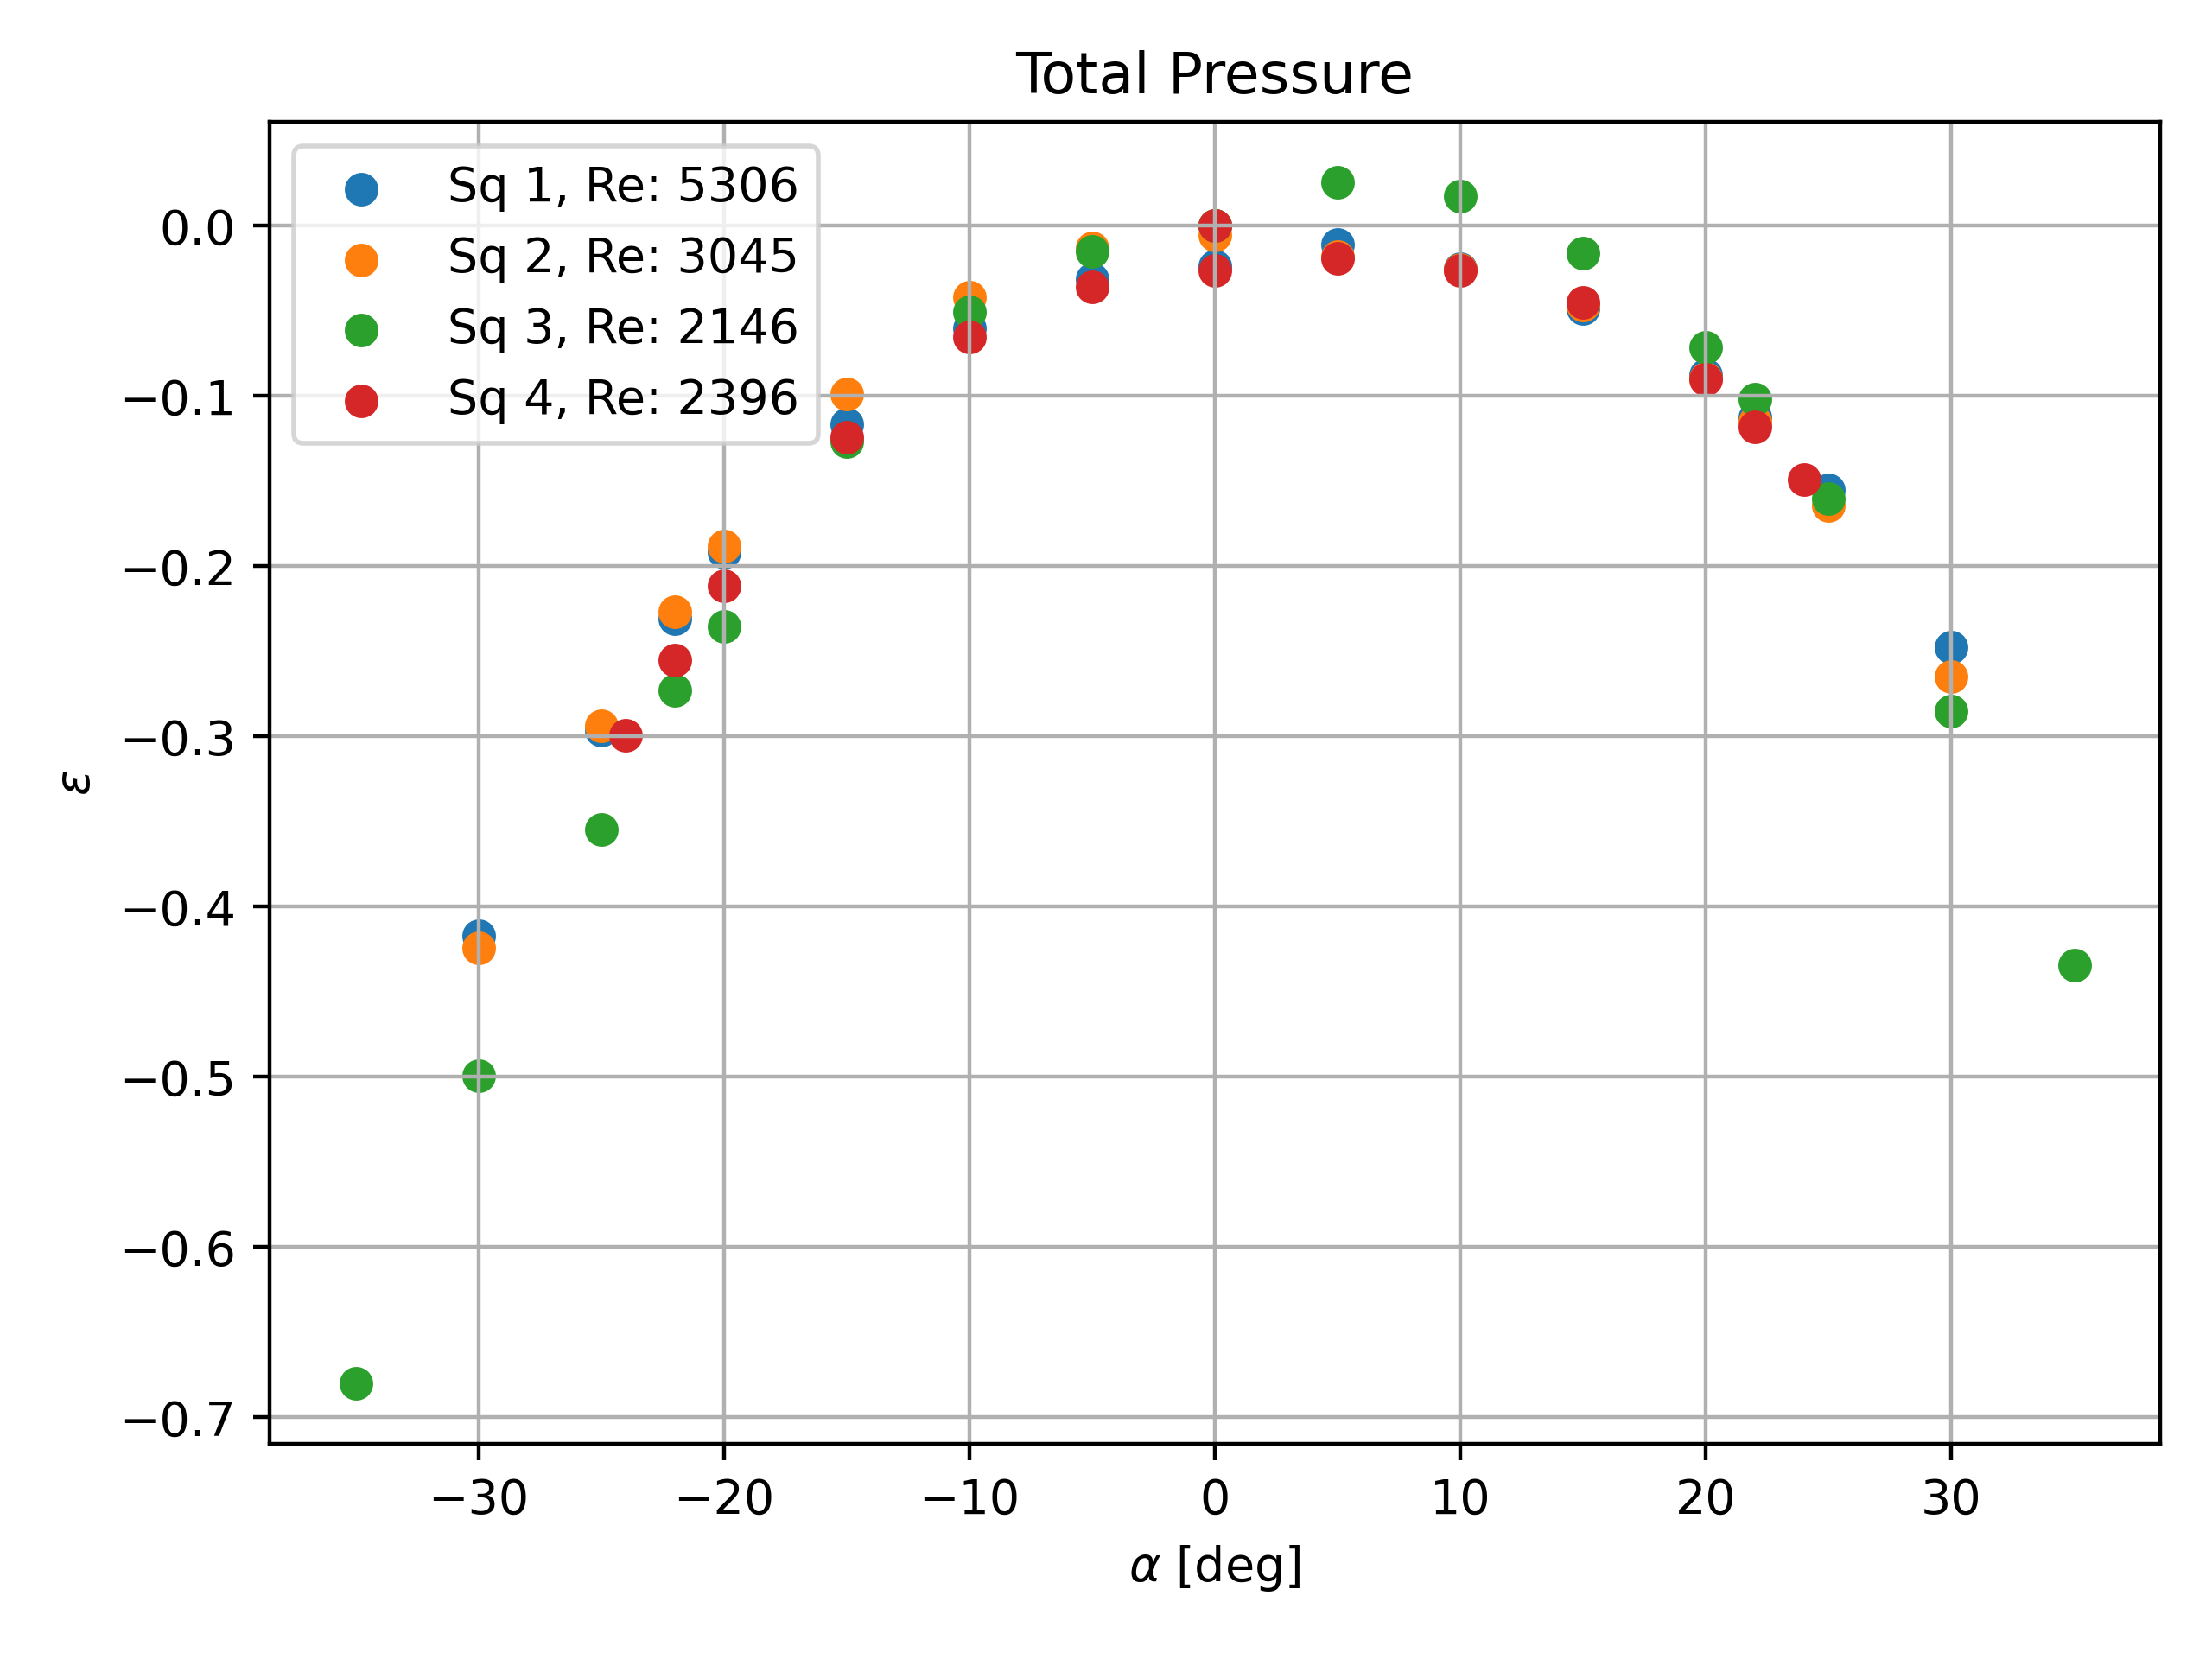
\includegraphics[width=.76\textwidth]{images/2/ptot.png}
    \caption{Pressione totale}
\end{figure}

\newpage
\begin{figure}[ht]
    \centering
    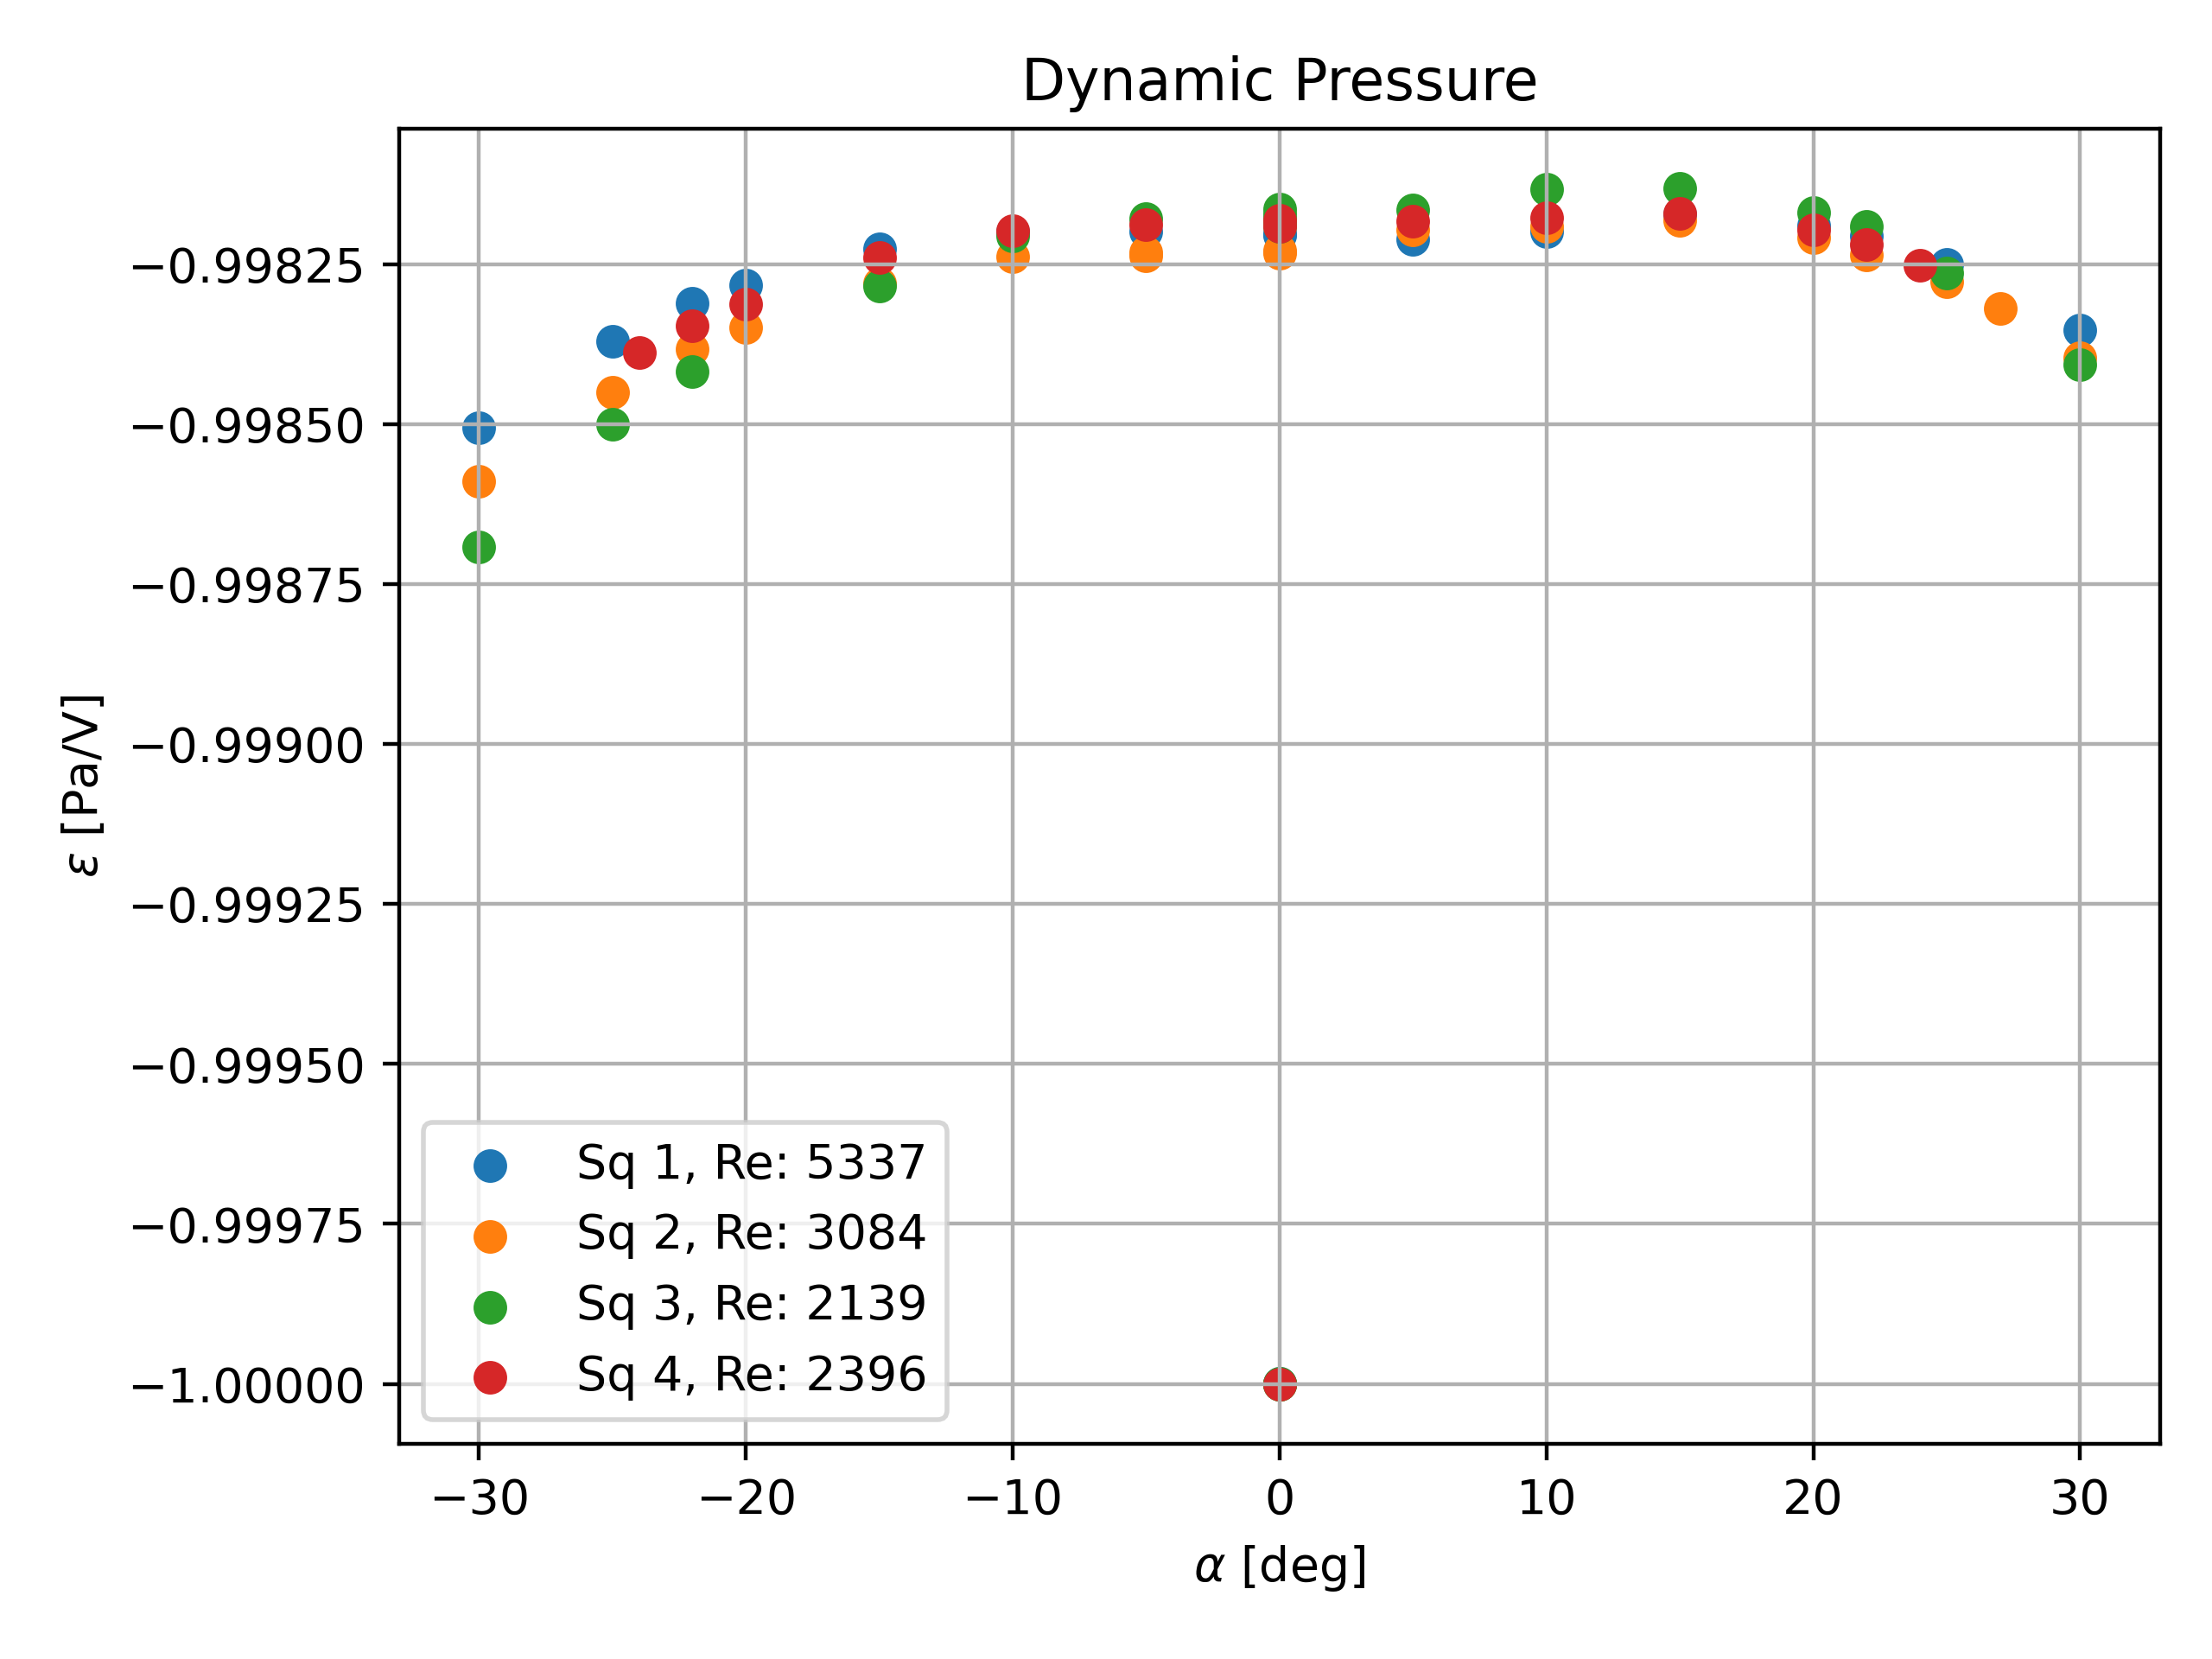
\includegraphics[width=.76\textwidth]{images/2/q.png}
    \caption{Pressione dinamica}
\end{figure}

\noindent I risultati ottenuti corrispondono ai diagrammi presenti in letteratura.\\\\
Dai risultati ottenuti non si evidenzia una particolare influenza dovuta alla variazione del numero di Reynolds.\\\\
Gli errori nel diagramma della pressione statica per la terza squadra risultano inferiori, probabilmente a causa di un errore sistematico durante la procedura sperimentale.\\\\
L'evidente asimmetria dei risultati, ottenuti variando all'angolo di disallineamento, è attribuibile all'interferenza dovuta al gambo della sonda di Pitot. Per ovviare a tale problematica sarebbe stato sufficiente orientare il gambo della sonda in direzione normale al piano di rotazione.

\newpage
\subsection{Tempo caratteristico}
A differenza dell'esercitazione precedente, nell'attuale catena di misura non è presente il manometro di Betz, che operava da collo di bottiglia per la risposta in frequenza della linea pneumatica. Pertanto, è opportuno indagare il fenomeno transitorio della linea pneumatica ed il relativo tempo caratteristico $\tau$.\\\\
Per fare ciò, sono acquisite le tensioni di uscita dal trasduttore con una frequenza di campionamento $f_{samp}=500$ Hz per un periodo $T$ di 2 minuti.\\\\
Per determinare il tempo caratteristico si interpolano i dati sperimentali con una curva esponenziale, del tipo:
\begin{equation*}
    E(t) = Ae^{bt} = Ae^{-\frac t\tau}
\end{equation*}
Maneggiando tale relazione, si ottiene:
\begin{equation*}
    \log E(t) = \log A + bt = c_1 t + c_2 \quad \Rightarrow \quad b = -\frac1\tau = c_1 \ ; \ A = e^{c_2}
\end{equation*}
Si ricava dunque il tempo caratteristico della linea pneumatica:
\begin{equation*}
    \tau = 0.400\ \text{s}
\end{equation*}
\begin{figure}[H]
    \centering
    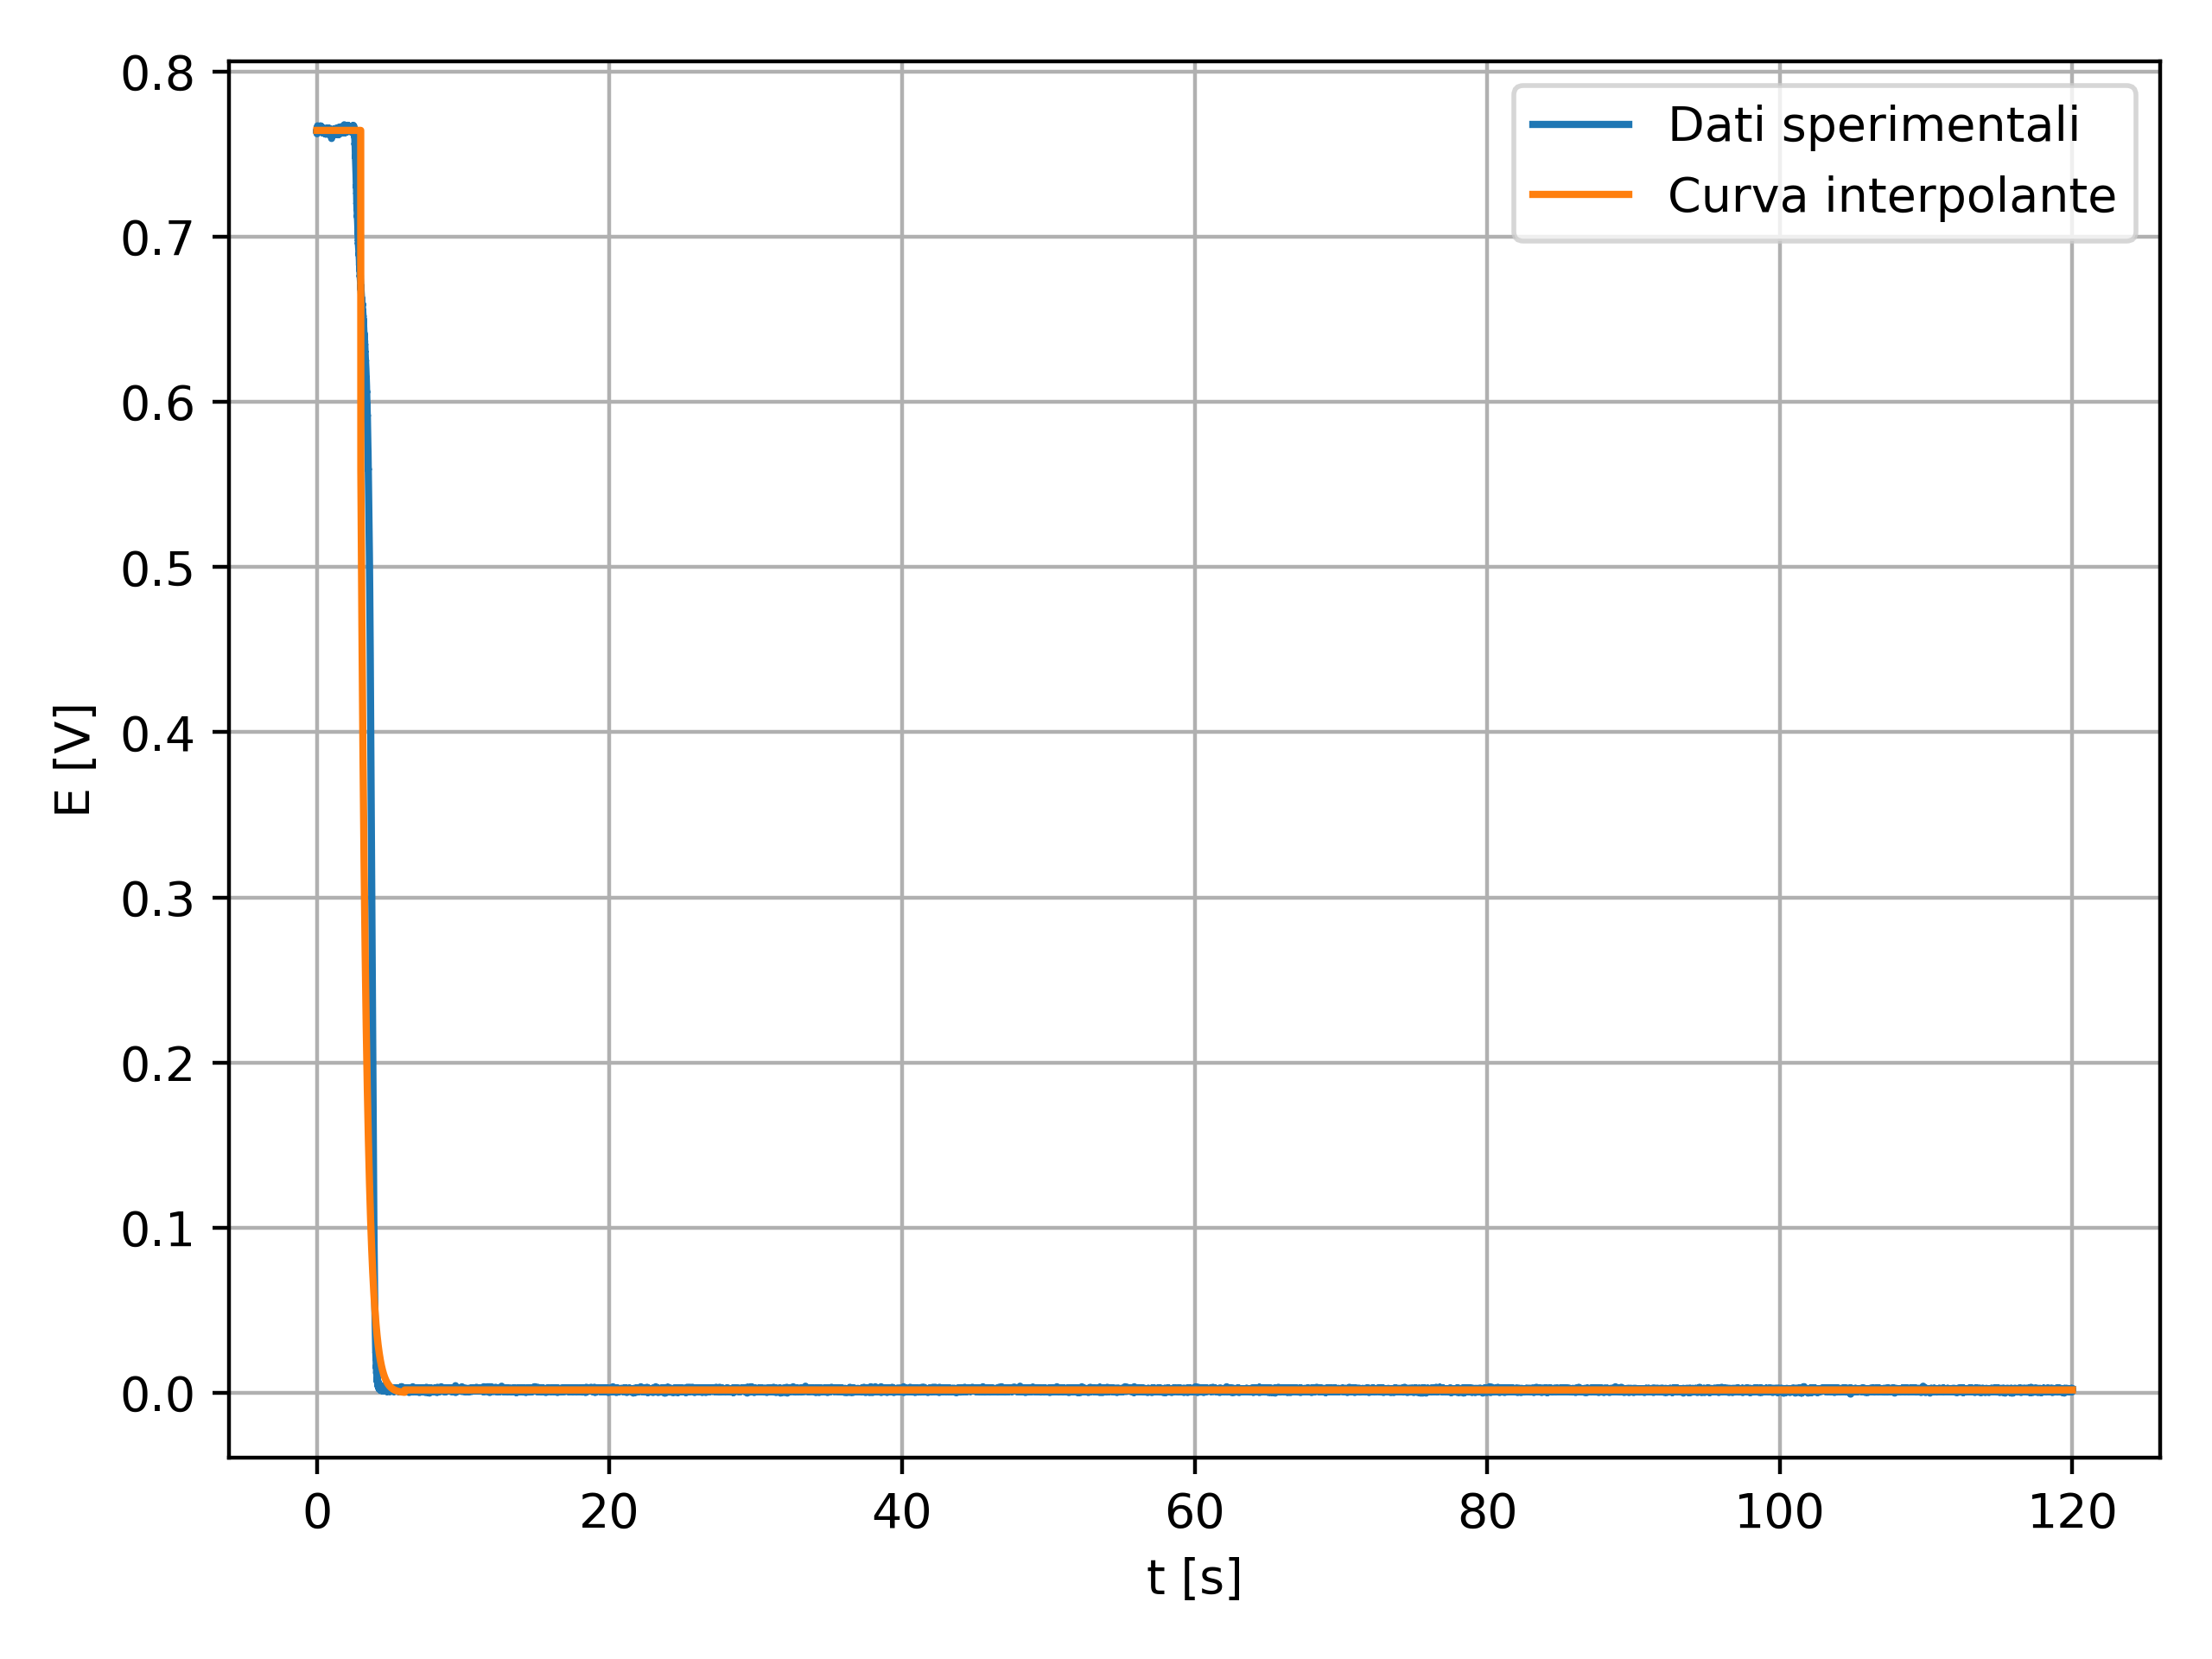
\includegraphics[width=.9\textwidth]{images/2/transitorio.png}
    \caption{Transitorio relativo alla pressione dinamica $q(t)$}\label{fig:t2}
\end{figure}